\documentclass[a4paper]{article}

\usepackage{tikz}
\usepackage{pgfplots}

\usepackage[english]{babel}
\usepackage[utf8]{inputenc}
\usepackage{amsmath}
\usepackage{graphicx}

\title{Finding a Minimum-Weight Spanning Tree Using Gallager, Humblet and Spira's Algorithm}

\author{Jens de Waard \\ 4009215 \and Tim Wissel \\ 4xxxxxx}

\date{\today}
\begin{document}


\maketitle
\begin{abstract}
Enter a short summary here. What topic do you want to investigate and why?
What experiment did you perform? What were your main results and
conclusion?
\end{abstract}

\section{Introduction}
\label{sec:introduction}
For exercise 3 of the course Distributed Algorithms we implemented the
algorithm by Gallager, Humblet and Spira for determining a minimum-weight
spanning tree of a distributed network. In this report we describe the
details of our implementation in section \ref{sec:implementation} and the
results of running the algorithm on two types of networks, manually and
automatically created, are listed in section \ref{sec:results}.

\section{Implementation}
\label{sec:implementation}
We've chosen to implement the algorithm in Java RMI. This was a requirement for
the previous assignments and as such we already had some code to work with. Had
we chosen to implement the algorithm in Python, we would have had to start from
scratch.

The implementation adds artificial delays when sending a message to simulate
the latency that occurs on true networks. Due to this delay, it is possible
that two messages send in quick succession over the same edge do not arrive in
the proper order; the later message will overtake the first. This is a
violation of the FIFO property of the network that the algorithm depends upon.

To counteract this, all messages are timestamped using a scalar clock that is
mainted by every node for each of its outgoing edges. Each node also maintains
for every incoming edge what the timestamp of the next message must be. Any
message that has a higher timestamp than expected is deferred until all prior
messages on the corresponding edge are received.

\subsection{Generation of test cases}
Creating large networks by hand would be very difficult and error-prone. Due to
this we created a bash script to output valid graphs that could be read by the
implementation. The script created graphs of sizes ranging from 5 to 100 nodes
in steps of 5 with a chance $p$ of an edge between each possible pair of nodes,
which $p \in \{0.25, 0.5, 1\}$. For each combination of size and $p$, 5 test
cases were created. However this didn't matter for when $p = 1$ as all
fully-connected graphs of size $n$ are equal. In those cases, there is still
additional value in having multiple tests as there is a certain randomness in
the implementation due to the delays and the specific node that starts the
algorithm.

\section{Results}
\label{sec:results}

Figure \ref{fig:message-plots} shows the relationship between the number of
nodes in a graph and the total number of messages sent by the algorithm. The
blue line corresponds to the number of messages that our implementation of the
algorithm sends, while the red line is the upper bound to the number of
messages as described by Gallager, Humblet and Spira in their paper. This
upper bound is $O(5 * n \log n + 2 E)$.

For higher values of $n$, the implementation sends more messages than the
expected upper bound would allow. This is especially noticable in the fully
connected networks.

\begin{figure*}[!t]
\centering
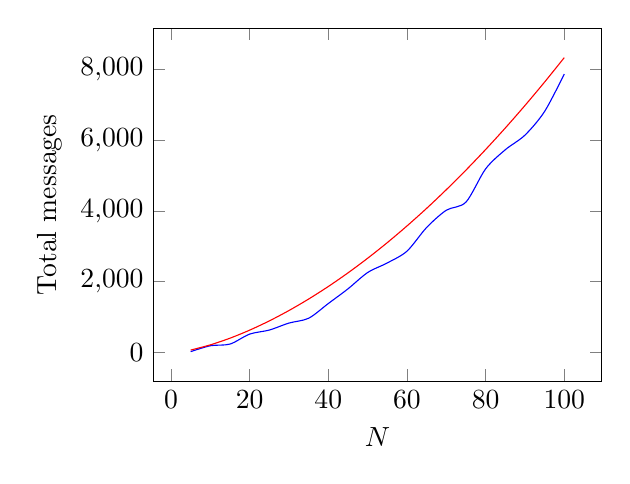
\begin{tikzpicture}
    \begin{axis}[
      height=0.5\textwidth,
      width=0.6\textwidth,
      xlabel=$N$,
      ylabel=Total messages
    ]
	
    \addplot[smooth ,color=blue] coordinates {
    	(5, 24.5)
		(10, 191.5)
		(15, 239)
		(20, 520.5)
		(25, 634.5)
		(30, 832)
		(35, 968)
		(40, 1383)
		(45, 1797.5)
		(50, 2257.5)
		(55, 2529)
		(60, 2860.5)
		(65, 3529)
		(70, 4015.5)
		(75, 4245.5)
		(80, 5183)
		(85, 5722.5)
		(90, 6135)
		(95, 6803.5)
		(100, 7859)
    };
	\addplot[smooth ,color=red] coordinates {
    	(5, 70.5)
		(10, 216.5)
		(15, 405)
		(20, 632)
		(25, 893)
		(30, 1186)
		(35, 1510)
		(40, 1864)
		(45, 2248)
		(50, 2661)
		(55, 3102)
		(60, 3572)
		(65, 4069)
		(70, 4595)
		(75, 5148)
		(80, 5729)
		(85, 6336)
		(90, 6971)
		(95, 7633)
		(100, 8322)
    };
    \end{axis}
\end{tikzpicture}

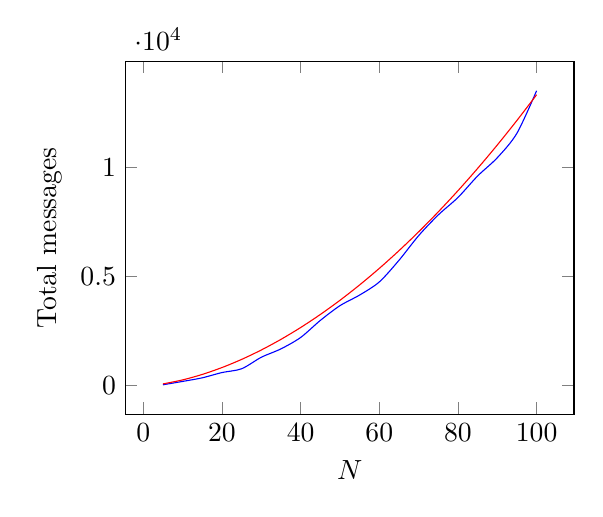
\begin{tikzpicture}
    \begin{axis}[
      height=0.5\textwidth,
      width=0.6\textwidth,
      xlabel=$N$,
      ylabel=Total messages
    ]
	
    \addplot[smooth ,color=blue] coordinates {
    	(5, 43)
		(10, 197)
		(15, 362)
		(20, 603)
		(25, 777)
		(30, 1303)
		(35, 1688)
		(40, 2209)
		(45, 2989)
		(50, 3665)
		(55, 4152)
		(60, 4751)
		(65, 5741)
		(70, 6870)
		(75, 7820)
		(80, 8618)
		(85, 9602)
		(90, 10438)
		(95, 11560)
		(100, 13506)
    };
	\addplot[smooth ,color=red] coordinates {
		(5, 83)
		(10, 266)
		(15, 518)
		(20, 832)
		(25, 1205)
		(30, 1636)
		(35, 2123)
		(40, 2664)
		(45, 3261)
		(50, 3911)
		(55, 4615)
		(60, 5372)
		(65, 6182)
		(70, 7045)
		(75, 7961)
		(80, 8929)
		(85, 9949)
		(90, 11021)
		(95, 12146)
		(100, 13322)
    };
    \end{axis}
\end{tikzpicture}

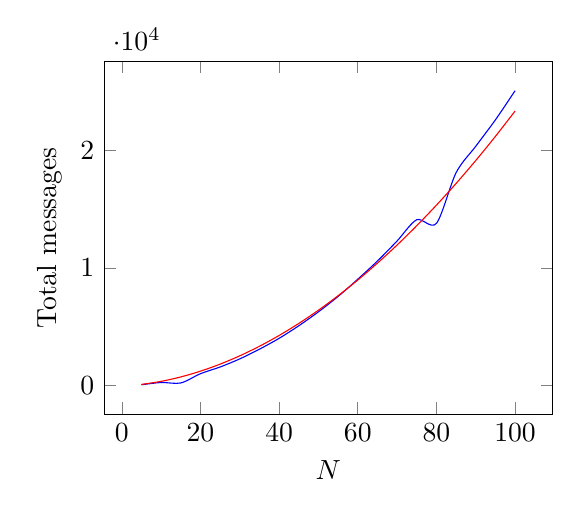
\begin{tikzpicture}
    \begin{axis}[
      height=0.5\textwidth,
      width=0.6\textwidth,
      xlabel=$N$,
      ylabel=Total messages
    ]
	
    \addplot[smooth ,color=blue] coordinates {
    	(5, 77)
		(10, 270)
		(15, 232)
		(20, 1019)
		(25, 1587)
		(30, 2277)
		(35, 3099)
		(40, 4021)
		(45, 5088)
		(50, 6271)
		(55, 7579)
		(60, 9043)
		(65, 10587)
		(70, 12290)
		(75, 14092)
		(80, 13786)
		(85, 18087)
		(90, 20331)
		(95, 22574)
		(100, 25046)
    };
	\addplot[smooth ,color=red] coordinates {
		(5, 108)
		(10, 366)
		(15, 743)
		(20, 1232)
		(25, 1830)
		(30, 2536)
		(35, 3348)
		(40, 4264)
		(45, 5286)
		(50, 6411)
		(55, 7639)
		(60, 8972)
		(65, 10407)
		(70, 11945)
		(75, 13586)
		(80, 15329)
		(85, 17174)
		(90, 19121)
		(95, 21171)
		(100, 23322)
    };
    \end{axis}
\end{tikzpicture}
\caption{The total number of messages and the expected number of messages for
$p = 0.25$, $p = 0.5$ and $p=1$.}
\label{fig:message-plots}
\end{figure*}


\section{Conclusion}
\label{sec:conclusion}

\begin{thebibliography}{9}
\bibitem{nano3}
  K. Grove-Rasmussen og Jesper Nygård,
  \emph{Kvantefænomener i Nanosystemer}.
  Niels Bohr Institute \& Nano-Science Center, Københavns Universitet

\end{thebibliography}
\end{document}
